%!TEX root = ../main.tex
\chapter{Implementation}
\section{Overview}
This section will describe how the features were implemented to develop the final artefact, the system will be developed using Android studio. 

\begin{figure}[h!]
	\centering       
	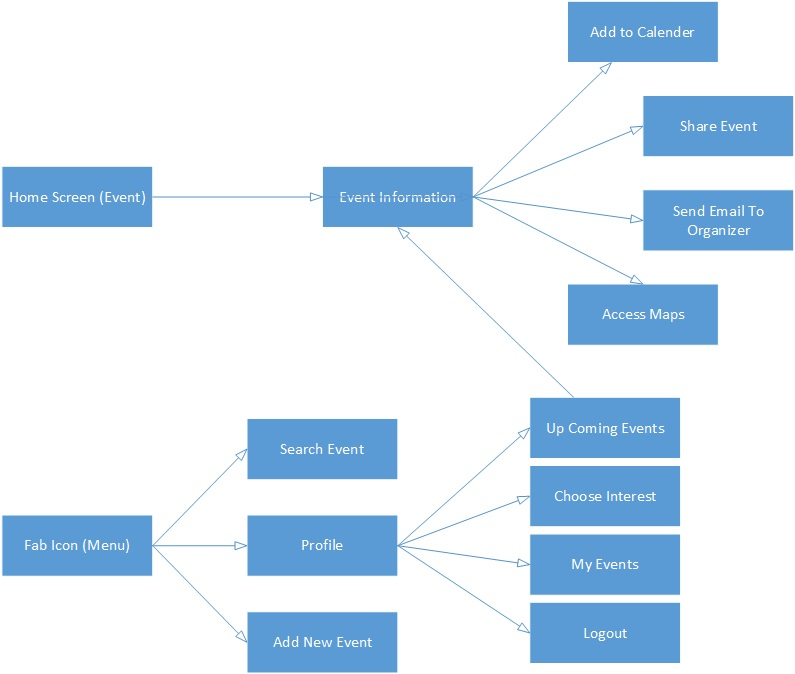
\includegraphics[width=0.35\textheight]{navigation_screens}
	\caption{Logic Flow of Screen}
	\label{fig:navigation_screen}	
\end{figure}
The figure above \ref{fig:navigation_screen} shows the relationship between each activity(screen), how to move between screens.
Both screens, upcoming event and homescreen link back to event information, because this option is available from both activities, meaning the user can access event information from both.
Add to calender, share event, send email to organizer and access maps are all behind event information, this means the logic behind each of those activities has to be implemented in the event information activity.
Fab icon, refer to figure \ref{fig:fab_menu}, is a navigation menu that links to search event, profile and add new event.
\begin{figure}
	\centering
	\begin{subfigure}[b!]{0.25\textwidth}  	      
		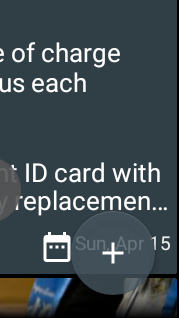
\includegraphics[width=.96\linewidth]{fab_menu_not_clicked}
		\caption{Fab Not Clicked}
		\label{fig:fab_not_clicked}
	\end{subfigure}%
	%add desired spacing between images, e. g. ~, \quad, \qquad etc.
	%(or a blank line to force the subfigure onto a new line)
	\begin{subfigure}[b!]{0.25\textwidth}	
		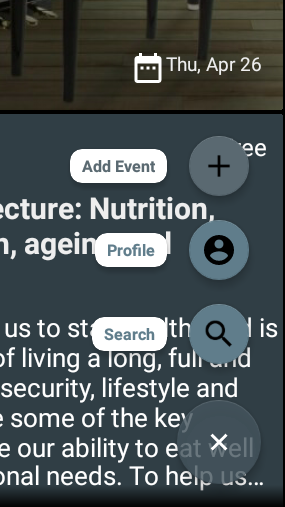
\includegraphics[width=.96\linewidth]{fab_menu_clicked}
		\caption{Fab Clicked}
		\label{fig:xml_editor}
	\end{subfigure}
	\caption{Fab Menu}\label{fig:fab_menu}
\end{figure}

\section{Login \& Register}
The login.xml has the function to display the views to the user while the login activity has the function to handle all the java logic in the background. This activity will ask the user to login, user then has to select their university, enter university email and password, this information is then checked against the user database; if the user has already got an account and the password is correct the user will be logged in successfully. This activity also checks if the user account is verified or not and displays the appropriate message. The user can move from the login activity to the Register activity by clicking on the textview, "not registered". Refer to appendix \ref{screen_design}, for details on screen design.

Activities relies on intent, refer to Appendix \ref{additional_components}, to move from one activity to the other, the figure below \ref{fig:intent} shows an example of how to move from the login activity to the register activity. Intent also allows data passage between activities; for the purposes of this app data such as user email, user ID, was passed through activities to maintain traceability.
\begin{figure}[h!]
	\centering       
	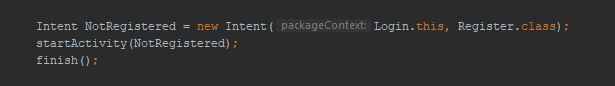
\includegraphics[width=0.5\textheight]{login_to_register}
	\caption{Declaring an Intent}
	\label{fig:intent}	
\end{figure}
In order to enhance the user experience, shared preferences APIs was used to store user login details on their phone(internal memory of the phone). Shared preferences permits saving and retrieving key value pair data to be used to save primitive data type such as Boolean, string, int, long and float.

\textbf{MODE\_PRIVATE} – this is the most used mode of sharedPreferences, It is a default mode, which means that when any preference file is created it will only be accessible from the application.

Calling the edit() function of SharedPreferences class which returns Editor class object allows to save data into sharePreferences, refer to figure \ref{fig:save_share_preferences}

\begin{figure}[h!]
	\centering       
	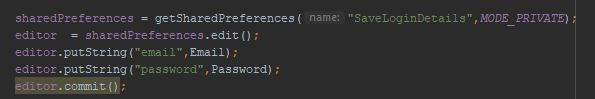
\includegraphics[width=0.5\textheight]{save_sharepreferences}
	\caption{Declaring SharePreferences}
	\label{fig:save_share_preferences}	
\end{figure}

Values stored in shared preferences can be called using SharedPreferences object by calling different primitive type function starting with get plus the Primitive type name, refer to figure \ref{fig:get_share_preferences}
\begin{figure}[h!]
	\centering       
	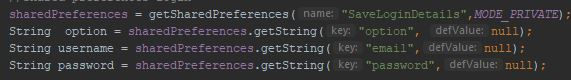
\includegraphics[width=0.5\textheight]{get_sharedpreferences}
	\caption{SharePreferences key value pair data}
	\label{fig:get_share_preferences}	
\end{figure} 
 
 The \textbf{register activity}  allows the user to create an account if they are not previously registered. It prompts the user to enter their details, university name, nickname, email and password. Afterwards, before registering the user, it verifies if the user does not have a previous account, if so it will displays a message. Otherwise it creates an account and sends a verification email to the users email address to verify their account, refer to appendix \ref{screen_design}.
 
 Once the user is registered and logged in, the app receives all the event data from the server and displays it on the home screen.

\section{Implementation of REST API}
REST stands for "Representational State Transfer" REST architecture will be used to build the client/server applications. It's simple to implement REST as it basically works on HTTP protocol, refer to figure \ref{fig:http_methods} below.
\begin{figure}[h!]
	\centering       
	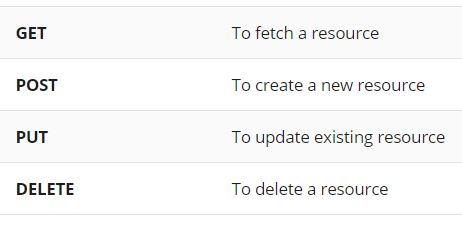
\includegraphics[width=0.5\textheight]{http_methods}
	\caption{HTTP Methods}
	\label{fig:http_methods}	
\end{figure} 

Since Android does not have a dedicated library for implementing A REST API, it provides a number of pre-implemented solutions that can be used for the implementation. According to \cite{kwon2016design}, the main issue however, is how to design an action
flow between components of the system from the presentation layer (Activities) down to the network and local memory operations.
He also mentions that there is nothing like the best way of implementing a RESTful API client on Android platform
because each solution can, and should be modified according to the unique requirements
of the protocol, however, there is one pattern which is definitely not advised, that is to, avoid running RESTful methods directly from the UI thread.
\begin{itemize}
	\item this would cause and ANR (Application Not Responding error). 
	\item slow down the application and make it less responsive 
\end{itemize}  

 Android however provides a solution, AsyncTask, which is a high-level concurrent construct. AsyncTask can interact with the UI thread by updating the UI via event handlers. For example, the event handler \textbf{\textit{onPostExecute}} executes after the task is finished, and can update the UI with the task results.
 A study by, \cite{7372076}, shows AsyncTask is the most used async construct in Android. However, it is designed for short-running tasks (i.e., less than one second) and if improperly used, can lead to memory leaks and lost results.
 
 The basic methods used in an android AsyncTask class are defined in the table below:
 
 
\begin{longtable}{| L{5cm} | L{9cm} |}
	Method  & Function  \\ \hline
doInBackground() & This method contains the code which will be executed in the background\\	\hline
	onPreExecute() &	This method contains the code which will be executed before the \textbf{\textit{doInBackground}} method\\	\hline
onProgressUpdate()   &This method receives progress updates from \textbf{\textit{doInBackground}} method\\	\hline
onPostExecute()  &	 This method is executed after \textbf{\textit{doInBackground}} completes processing and the result from \textbf{\textit{doInBackground}} is passed to this method\\	\hline
	\caption{AsynTask Methods}
	\label{methods}
\end{longtable}
\pagebreak
\subsection{Sending Request to the Server}
There are multiple networking libraries and classes available for Android that can send POST requests, however, the preferred method is through HttpUrlConnection.
This section will describe how to send request from Android client to the server;

\textbf{Giving Permission to Android:}
Univent requires an internet connection in order to get information about the event and to retrieve data from the database. All required permissions must be declared in the AndroidManifest.xml file.
\begin{figure}[h!]
	\centering       
	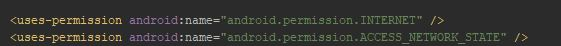
\includegraphics[width=0.5\textheight]{permission_internet}
	\caption{Internet Permission}
	\label{fig:internet_permission}	
\end{figure} 

\textbf{Connecting to the Server using URL:} The URL object, refer to figure \ref{fig:urlObject}, contains all the necessary information to reach the destination resource. In this example, the url is pointing to the php file on the server, named get\_event.php. This file handles the query to get all events from the database.
URLs are constructed as sets of information. Lets consider the URL:
\begin{center}
\textbf{ http://derton04.000webhostapp.com/login.php?parameter=value}
\end{center}

In the example above, http is the protocol, derton04.000webhostapp.com is the domain name, and login.php the path. Parameter a query parameter key (called key), value a query parameter value (named as value), and parameter=value a query parameter key-value pair (referred to as key-value pair).
\begin{figure}[h!]
	\centering       
	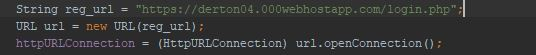
\includegraphics[width=0.5\textheight]{URL_GET_DATA}
	\caption{URL to get all Events in the Database}
	\label{fig:urlObject}	
\end{figure} 
 
 In the next step, \ref{fig:url_get}, the methods and properties of the request object are set. First, set the method as request method to be invoked as POST. The method setDoOutput, needs to be set to true before sending a post request. setDoOutput is not needed for GET requests.
  \begin{figure}[h!]
 	\centering       
 	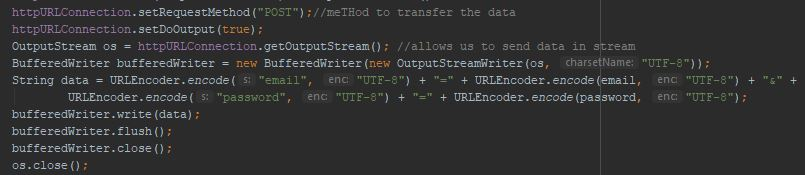
\includegraphics[width=0.5\textheight]{url_object}
 	\caption{URL to get all Events in the Database}
 	\label{fig:url_get}	
 \end{figure} 

 This library also gives the possibility of including data in the request. The URLConnection class provides an OutputStream object as the mechanism for providing this data, for performances reason it is wrapped in a buffered writer.
 The parameters/data are then attached to the url, then encoded onto the outPutStream before being transmitted over the internet.

The snippet below, figure \ref{fig:response_code} checks if the connection was successful and if the data has been transmitted.
\begin{figure}[h!]
	\centering       
	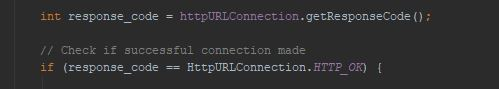
\includegraphics[width=0.4\textheight]{response_code}
	\caption{Check if Connection is OK}
	\label{fig:response_code}	
\end{figure}

 The figure below, \ref{fig:status_code}shows the status code of an http connection.
\begin{figure}[h!]
	\centering       
	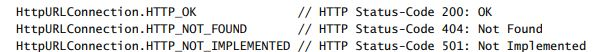
\includegraphics[width=0.4\textheight]{status_code}
	\caption{Status Code}
	\label{fig:status_code}	
\end{figure} 

 After receiving the Http status code OK, the URL will return some values that are directly coming from the database. Using inputStream and the String builder class, will fetch this data(JSON format) and store it in the variable, in this case result.
\begin{figure}[h!]
	\centering       
	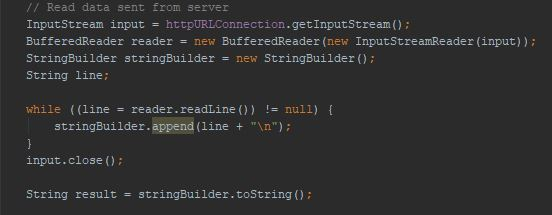
\includegraphics[width=0.4\textheight]{read_result_from_api}
	\caption{Status Code}
	\label{fig:read_result}	
\end{figure}

Figure \ref{fig:parse_json}, shows how the data is parsed using JSON parsing technique inside android application and then set into recycleview. 
\begin{figure}[h!]
	\centering       
	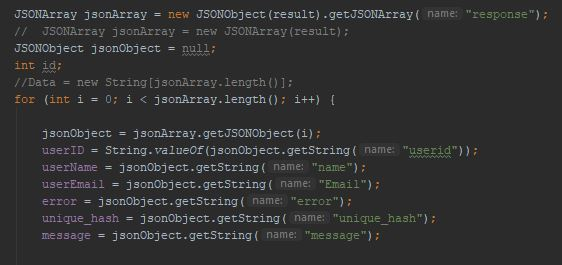
\includegraphics[width=0.4\textheight]{get_json}
	\caption{Parsing JSON}
	\label{fig:parse_json}	
\end{figure}
\pagebreak
To access the database, it requires an interface, first, it must receive JSON data, add data and update the database, secondly, it
must deliver JSON data containing events in the database.
A PHP scripts is used to provide this interface, below is a complete example of connecting an android application with MYSQL database via PHP script. It creates a basic application that retrieves data from MYSQL database using GET and POST method.

The PHP page given below takes parameters(userid) by POST method, and displays all event in the database created by that userID. The result will be displayed in JSON format.
\begin{figure}[h!]
	\centering       
	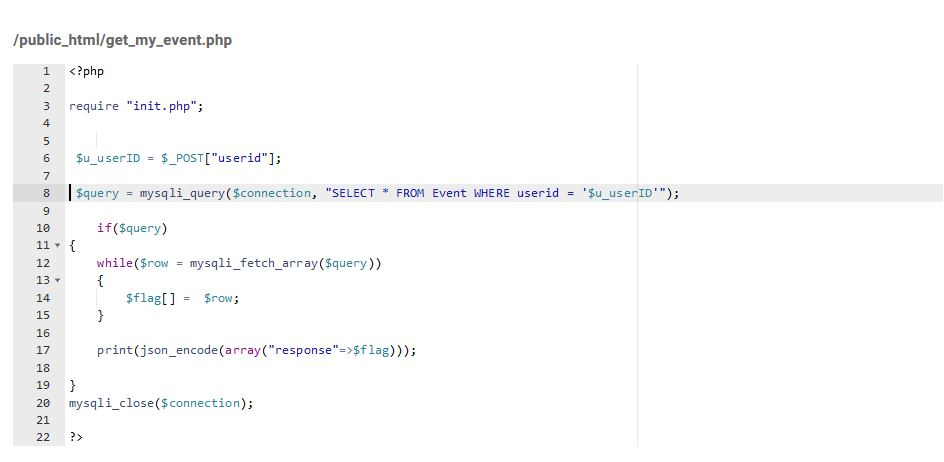
\includegraphics[width=0.5\textheight]{php_code}
	\caption{PHP Page}
	\label{fig:php_code}	
\end{figure}
The PHP file is responsible for handling the communication with the database, to insert, update, retrieve and delete data. To do so, the query is embedded in the PHP file which is then capable of establishing the connection with the MySQL database and execute the required query.

\textbf{JSON -}
JSON (JavaScript Object Notation)  is a lightweight text-data interchange format used to transmit data in form of objects(structured data: key value pairs) over the internet. JSON also supports string, Boolean, number, array and null formats for storing data.
After the database operation is done, the server will save the result as JSON format, and send it to the requesting client, refer to Appendix \ref{json} for an example of JSON data format.

\section{Sending Image to Server}
\label{sending_image_server}
This section explains how the images  of each event were uploaded to the server using the Volley library, see Appendix \ref{sending_image_server_appendix}.

\section{Testing}
To ensure the system was tested thoroughly a test suit was designed.
Test results are shown is Appendix \ref{appendix:test_suit}.
\subsection{System Testing}
The purpose of system testing is to test Univent against the functional requirements declared in section \ref{req_analysis}.
Appendix \ref{appendix:test_suit} detail the system testing.

\subsection{Black Box Testing}
Android app must be tested on the emulators, but it is important to test the app in the real world. The app has been constantly been tested from initial installation to daily use of app as per the end users point of view. This method is more powerful to come to know if any issues become visible in Android apps, as issues will surface in day to day use.

After each new functionality added, a thorough testing is done by the author, the supervisor and some experimental users. 
This method resulted in being very effective as some defects, with varying severity, were identified, for example, the send email button in the event information page, was meant to send an email to the event host, instead it was sending the email to the actual user. 
Another behaviour identified that was very crucial, was the login validation, user were allowed to register with a blank password, therefore they could login  without typing in the password. 

\section{Publishing to Play Store}
After all testing has been completed, the application was
published on the Google Play Store. 
The app was released on the Android Market under the name Univent and it will be free for all users. 